\subsubsection{Data Sources}
\label{sec:ui_configure_data_sources}

The 'Data Sources' group lists all data sources of the active Data Context, grouped by DSType (e.g. 'Radar', 'ADS-B', 'MLAT', 'Tracker'). Selecting a data source in the tree opens the data-source edit widget on the right. \\

\begin{figure}[H]
  \center
  \hspace*{-1cm}
    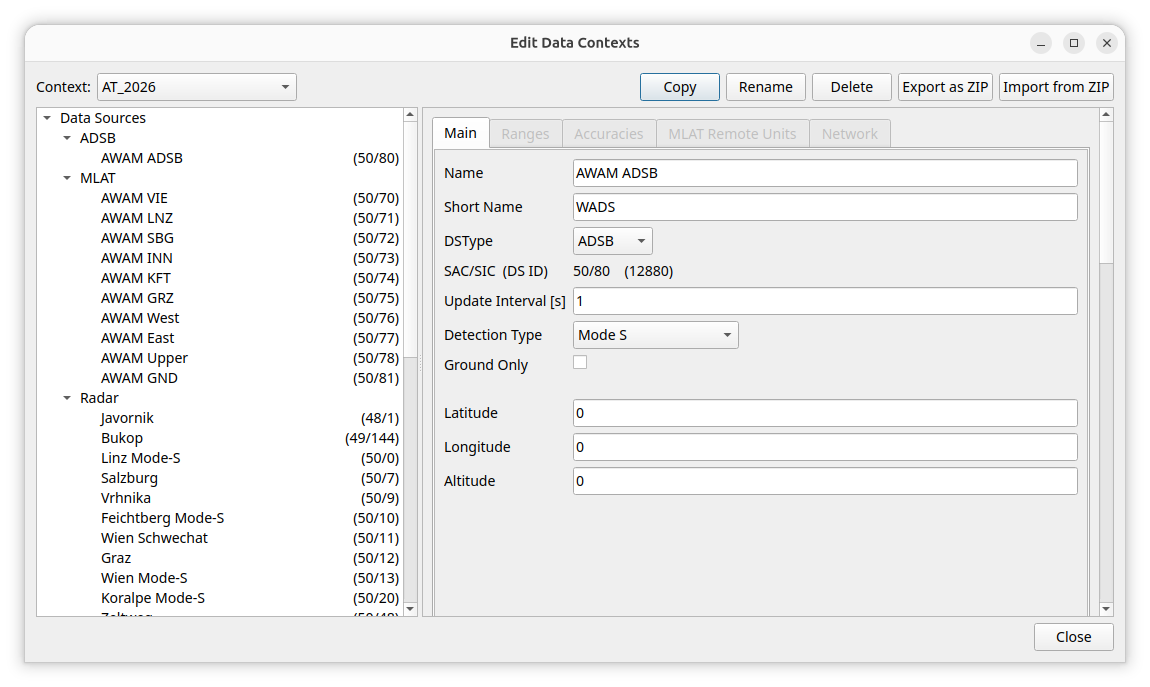
\includegraphics[width=17cm]{figures/data_context_edit_ds.png}
  \caption{Data Context: Data Source detail widget}
\end{figure}

A data source is always stored in the active Data Context, which means it is persistent across databases that share the same context. It is useful to define all existing data sources up front, since they are immediately picked up during import of data. A data source is additionally stored in the database only if data from said source is imported. During the import, if a data source can be found (matching SAC/SIC) in the active context, it is automatically attached to the database. \\

Please \textbf{note} that the position of a data source is only required for sources of DSType 'Radar' (used by the radar plot position calculation). For all other DSTypes, SAC/SIC and name information are sufficient for display purposes. \\

However, for CAT010, CAT020 and CAT062 the option exists to project from a Cartesian X/Y coordinate system to WGS84 latitude and longitude (when not available in the ASTERIX data). To use this feature during ASTERIX import, a latitude and longitude have to be set on the respective data source. \\

The detail widget contains the following tabs:

\begin{itemize}
\item Main: Main attributes (always shown)
\item Network Lines: Network configuration for ASTERIX network import (always shown)
\item Radar Ranges: Optional detection ranges (shown for DSType 'Radar')
\item Radar Accuracies: Optional accuracy information (shown for DSType 'Radar')
\item MLAT Remote Units: Optional Remote Unit definition for Contributing Receivers analysis (shown for DSType 'MLAT')
\end{itemize}
\ \\

\paragraph{Tree Actions}

Right-clicking the 'Data Sources' group offers:

\begin{itemize}
\item Add Data Source...: Opens a small dialog with SAC, SIC and DSType fields and creates a new data source from the entered values
\item Import...: Imports configuration data sources from a JSON file (see \nameref{sec:config_ds_export})
\item Export...: Exports all data sources of the active context as a JSON file
\item Delete All: Removes all data sources from the active context after a confirmation prompt (disabled if any source already has data in the database)
\end{itemize}
\ \\

Right-clicking a single data source offers a 'Delete' action, which is disabled if the source already has data in the database. \\

\paragraph{Main Tab}

Depending on the DSType, additional fields are shown. For all sources, the following information is given:

\begin{itemize}
\item Name: Name of the data source
\item Short Name: Short name of the data source (optional)
\item DSType: Data source type, e.g. 'Radar', 'MLAT', 'ADS-B', ...
\item SAC/SIC (DS ID): System Area Code, System Identification Code, derived data source ID (256*SAC+SIC)
\item Detection Type: See below
\item Update Interval: Update interval in seconds (for correct labeling)
\item Ground Only: Check if the data source \textbf{only} provides detection for on-ground targets (e.g. for SMRs or local MLAT)
\end{itemize}
\ \\

For sources of DSType 'Radar', the following additional information should be provided:

\begin{itemize}
\item Latitude: Source center position as WGS-84 latitude, as a floating point number in degrees, e.g. 42.0001
\item Longitude: Source center position as WGS-84 longitude, as a floating point number in degrees, e.g. 17.01
\item Altitude: Source center altitude above MSL, in meters
\item Ignore Range/Azimuth values: Ignore such position information when set (e.g. if provided erroneously)
\end{itemize}
\ \\

\paragraph{Detection Type}

A detection type can be given for any data source; 'Unknown' is set as default. Currently only 'Primary Only' is evaluated during reconstruction, but it is very important to set this type for SMRs, to mitigate sub-optimal association of primary-only target reports in close distance to clutter. \\

\begin{figure}[H]
  \center
    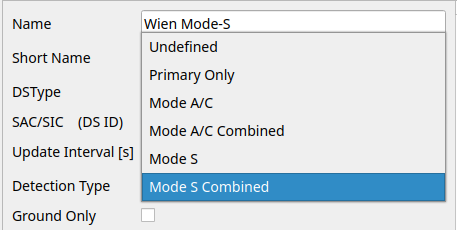
\includegraphics[width=10cm,frame]{figures/configure_ds_dettyp.png}
  \caption{Data Source: Detection Type combo box}
\end{figure}

For primary-only data sources, additional JPDA settings can be provided for the reconstructor:

\begin{itemize}
\item JPDA PD [1]: Probability of Detection, e.g. 0.9 for 90\%
\item Clutter Rate [1]: Rate of clutter detections per update interval, e.g. 10 in the configured PSR maximum range (has to be set in the 'Radar Ranges' tab to take effect)
\end{itemize}
\ \\

\begin{figure}[H]
  \center
    \includegraphics[width=10cm,frame]{figures/configure_ds_jpda.png}
  \caption{Data Source: JPDA fields}
\end{figure}

\paragraph{Network Lines Tab}
\label{sec:configure_datasources_network}

The 'Network Lines' tab defines up to 4 network lines (L1 to L4) per data source for ASTERIX network import. \\

\begin{figure}[H]
  \center
    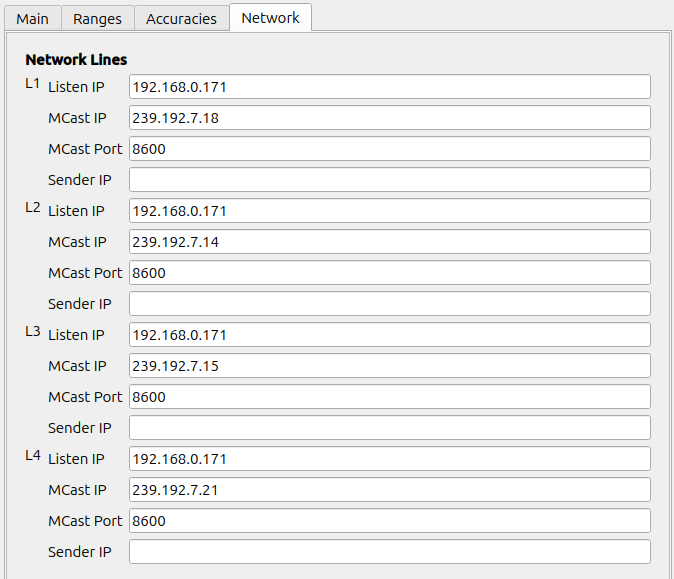
\includegraphics[width=14cm,frame]{figures/configure_network.png}
  \caption{Data Source: Network Lines tab}
\end{figure}

\begin{itemize}
\item 4 different lines are possible, each with:
\begin{itemize}
  \item Listen IP: Defines the used network interface and IGMP requests
  \item Multicast IP
  \item Multicast Port
  \item Sender IP: Optional, for filtering purposes
\end{itemize}
\end{itemize}
\ \\

Please \textbf{note} that for using real multicast addresses (inside of 224.0.0.0 to 239.255.255.255), it is recommended to also define the Listen IP as the local address of the network interface to be used. Otherwise the multicast data might not be received, or the wrong network interface might be picked up, causing COMPASS to receive no data. \\

Please also \textbf{note} that if e.g. only Multicast IP and port are set, and the Multicast IP is set to a non-multicast one (outside of 224.0.0.0 to 239.255.255.255), a local replay is possible (without real multi-casting). \\

\paragraph{Radar Ranges Tab}
\label{sec:configure_datasources_radar_ranges}

For DSType 'Radar', detection ranges can be configured per sensor type:

\begin{figure}[H]
  \center
  \hspace*{-1cm}
    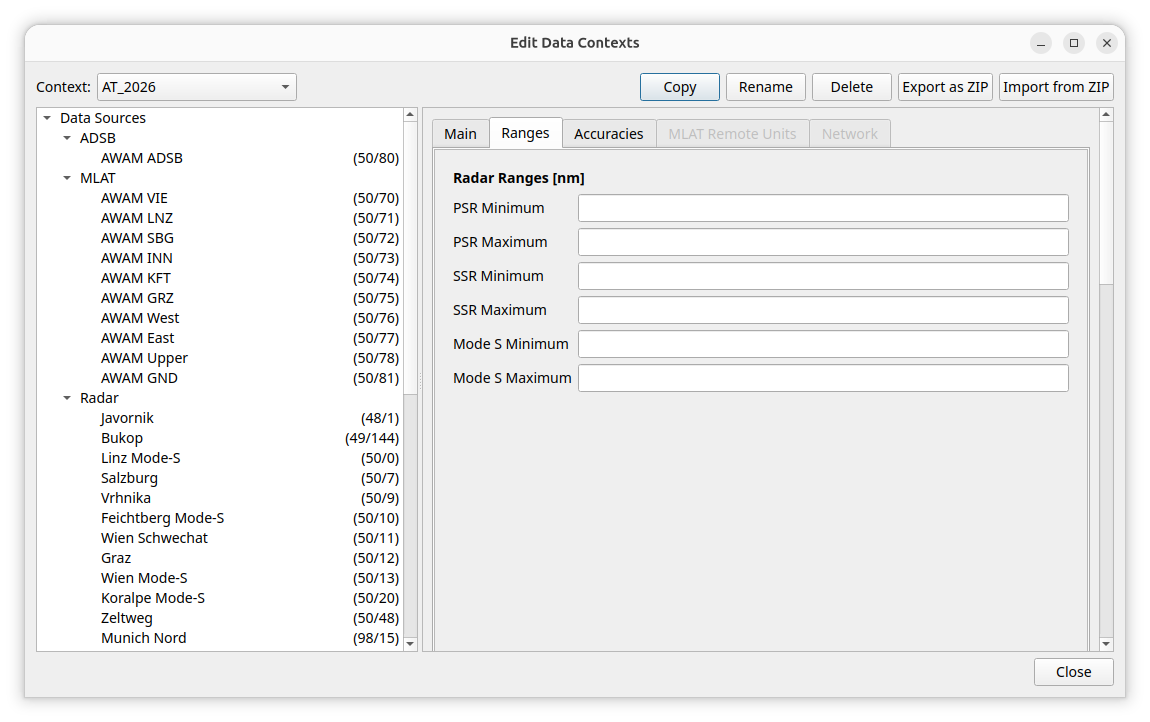
\includegraphics[width=17cm]{figures/data_context_edit_rad_range.png}  
  \caption{Data Source: Radar Ranges tab}
\end{figure}

\begin{itemize}
\item PSR Minimum: PSR minimum range, in nautical miles
\item PSR Maximum: PSR maximum range, in nautical miles
\item SSR Minimum: SSR minimum range, in nautical miles
\item SSR Maximum: SSR maximum range, in nautical miles
\item Mode S Minimum: Mode S minimum range, in nautical miles
\item Mode S Maximum: Mode S maximum range, in nautical miles
\end{itemize}
\ \\

\paragraph{Radar Accuracies Tab}

For DSType 'Radar', per-channel measurement accuracies (standard deviations) and, optionally, systematic radar errors (biases) can be configured: \\

\begin{figure}[H]
  \center
  \hspace*{-1cm}
    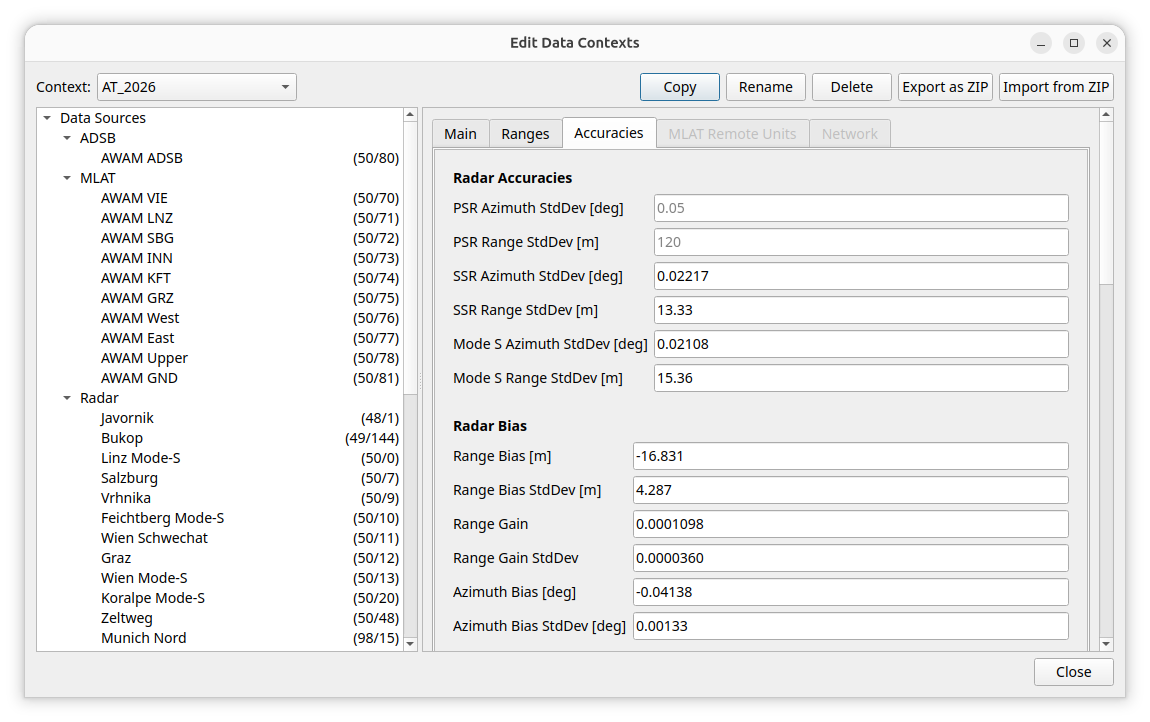
\includegraphics[width=17cm]{figures/configure_radar_accuracies.png}
  \caption{Data Source: Radar Accuracies tab}
\end{figure}

The 'Radar Accuracies' group defines the random measurement noise of the antenna per detection channel (PSR, SSR, Mode S):

\begin{itemize}
\item PSR Azimuth StdDev: PSR azimuth standard deviation, in degrees
\item PSR Range StdDev: PSR range standard deviation, in meters
\item SSR Azimuth StdDev: SSR azimuth standard deviation, in degrees
\item SSR Range StdDev: SSR range standard deviation, in meters
\item Mode S Azimuth StdDev: Mode S azimuth standard deviation, in degrees
\item Mode S Range StdDev: Mode S range standard deviation, in meters
\end{itemize}
\ \\

These values are used as a fall-back position accuracy for radar target reports without a reported accuracy, by projecting the polar standard deviations into a Cartesian covariance at the reported range and azimuth. They are consumed by both reconstructors during reference trajectory calculation, see \nameref{sec:reconst}. \\

In addition, systematic radar errors (biases) can be configured. The 'Radar Bias' group is hidden by default and shown after pressing the 'Add Radar Biases' button below the accuracies, which initializes all bias fields to zero:

\begin{itemize}
\item Range Bias [m]: Additive range offset, in meters
\item Range Bias StdDev [m]: Estimated uncertainty of the range bias, in meters
\item Range Gain: Multiplicative range scale error (unitless, e.g. 0.001 for a 0.1\% range stretch)
\item Range Gain StdDev: Estimated uncertainty of the range gain (unitless)
\item Azimuth Bias [deg]: Additive azimuth offset, in degrees
\item Azimuth Bias StdDev [deg]: Estimated uncertainty of the azimuth bias, in degrees
\end{itemize}
\ \\

If defined, these biases are applied during projection from polar radar measurements to Cartesian coordinates by both reconstructors when the 'Correct Radar Biases' option is enabled, see \nameref{sec:reconst}. \\

When the Probabilistic + IMM reconstructor is used, the biases are additionally estimated per radar Data Source from the available reference trajectory and written back into the active Data Context, so that the values shown in this tab reflect the latest estimate after each reconstructor run, see \nameref{sec:reconst_radar_bias_estimation}. \\

\paragraph{MLAT Remote Units Tab}
\label{sec:ui_configure_ds_mlat_rus}

For DSType 'MLAT' an additional 'MLAT Remote Units' tab is shown. It allows defining the list of contributing Remote Units (RUs) for the selected MLAT data source. \\

When no RUs are defined yet, the tab shows an empty-state placeholder with a dedicated 'Add Remote Units' button to start populating the list. Once at least one RU exists, the tab shows the RUs in a table and offers the 'Add', 'Import' and 'Remove All' buttons. \\

\begin{figure}[H]
  \center
    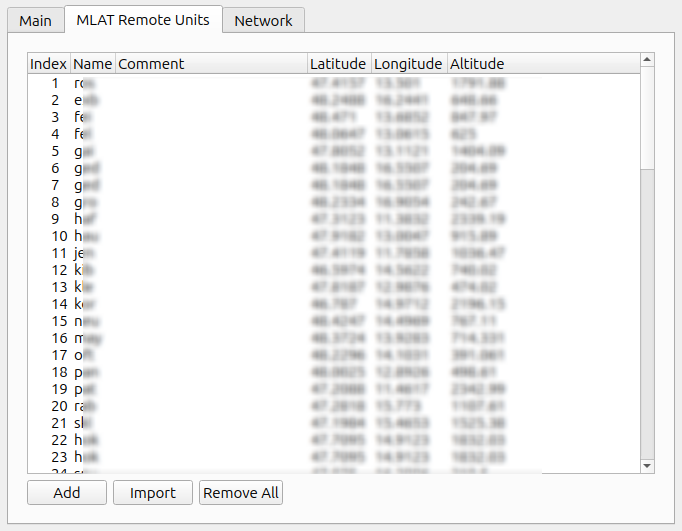
\includegraphics[width=12cm,frame]{figures/configure_mlat_rus.png}
  \caption{Data Source: MLAT Remote Units populated}
\end{figure}

The RU table has the following columns:
\begin{itemize}
\item Index: Number of the RU, starting with 1
\item Name: Short name of the Remote Unit
\item Comment: Optional comment
\item Latitude: WGS-84 latitude in degrees
\item Longitude: WGS-84 longitude in degrees
\item Altitude: Altitude in meters above MSL
\end{itemize}
\ \\

If defined, the information can be used in:
\begin{itemize}
\item DB Filters: Use names instead of indexes in the 'MLAT RUs' filter
\item Table View: Display names instead of indexes for 'Contributing Receivers'
\item Geographic View: Display of Remote Units and connection lines for target reports to each contributing receiver
\end{itemize}
\ \\

\paragraph{Add}

The 'Add' button opens a small dialog with fields for Index, Name, optional Comment, Latitude, Longitude and Altitude. Confirming the dialog appends one Remote Unit to the table. \\

\paragraph{Edit / Remove}

Right-clicking one or more rows in the table opens a context menu offering 'Edit' and 'Remove'.

\begin{itemize}
\item Edit: Opens the 'Edit Remote Unit' dialog with all fields editable except the Index
\item Remove: Deletes the selected row(s); multi-selection is supported
\end{itemize}
\ \\

\paragraph{Import}

The 'Import' button opens a file picker for a CSV file containing the full RU definition. \\


\includegraphics[width=0.5cm]{../../data/icons/hint.png} \textbf{Please note that importing replaces all existing Remote Units of the selected data source - existing entries are cleared before the file is parsed.} \\

The CSV file must have the following format:
\begin{itemize}
\item 6 columns: Index, Name, Comment, Latitude, Longitude, Altitude
\item Separator: ';'
\item Decimal point: '.'
\item Strings may be quoted with double quotes
\item Indices must be unique and \textbf{1-based}
\end{itemize}
\ \\

An MLAT RUs definition file shall be defined as follows:
\begin{lstlisting}
1;name1;"comment1";4.4157313889;1.5009816667;191.88
2;name2;;4.2488102778;1.2440838889;68.66
3;name3;"comment 3";4.4709594444;1.6851777778;87.97
\end{lstlisting}

\paragraph{Remove All}

The 'Remove All' button clears all defined Remote Units of the selected data source after a confirmation prompt.

\paragraph{Import/Export of Data Sources}
\label{sec:config_ds_export}

The 'Import...' and 'Export...' actions on the 'Data Sources' group's context menu read and write the data sources of the active context to and from a JSON file. There are 2 versions of the data sources JSON format used for import/export; please refer to \nameref{sec:appendix_data_sources}. \\

Using these actions, the data sources of one Data Context can be carried over to another (e.g. for sensor context switches, or to seed a new context from an exported file).
